%%%%%%%%%%%%%%%%%%%%%%%%%%%%%%%%%%%%%%%%%%%%%%
%                insertmeeting
% 1) Title (something creative & funny?)
% 2) Date (MM/DD/YYYY)
% 3) Location (ex. Hagerty High School)
% 4) People/Committees Present 
% 5) Picture 
% 6) Start Time & Stop Time (ex. 12:30AM to 4:30PM)
%%%%%%%%%%%%%%%%%%%%%%%%%%%%%%%%%%%%%%%%%%%%%%
\insertmeeting 
	{Velocity Vortexes (?)} 
	{01/04/22} 
	{Hagerty High School}
	{Anouska, James, Ritam, Samantha}
	{Images/RobotPics/robot.jpg}
	{2:30 - 4:30}
	
\hhscommittee{Software}
\noindent\hfil\rule{\textwidth}{.4pt}\hfil
\subsubsection*{Goals}
\begin{itemize}
    \item Develop a system to convert wheel velocities to a robot velocity.

\end{itemize} 

\noindent\hfil\rule{\textwidth}{.4pt}\hfil

\subsubsection*{Accomplishments}
We created a function in Kotlin named "wheelToRobotVelocities" that takes in wheelVelocities and steeringAngle as arguments. The function finds the left and right wheel velocities, then converts them to a robot velocity. The derviation of the formula can be found in the attached picture. 


\begin{figure}[htp]
\centering
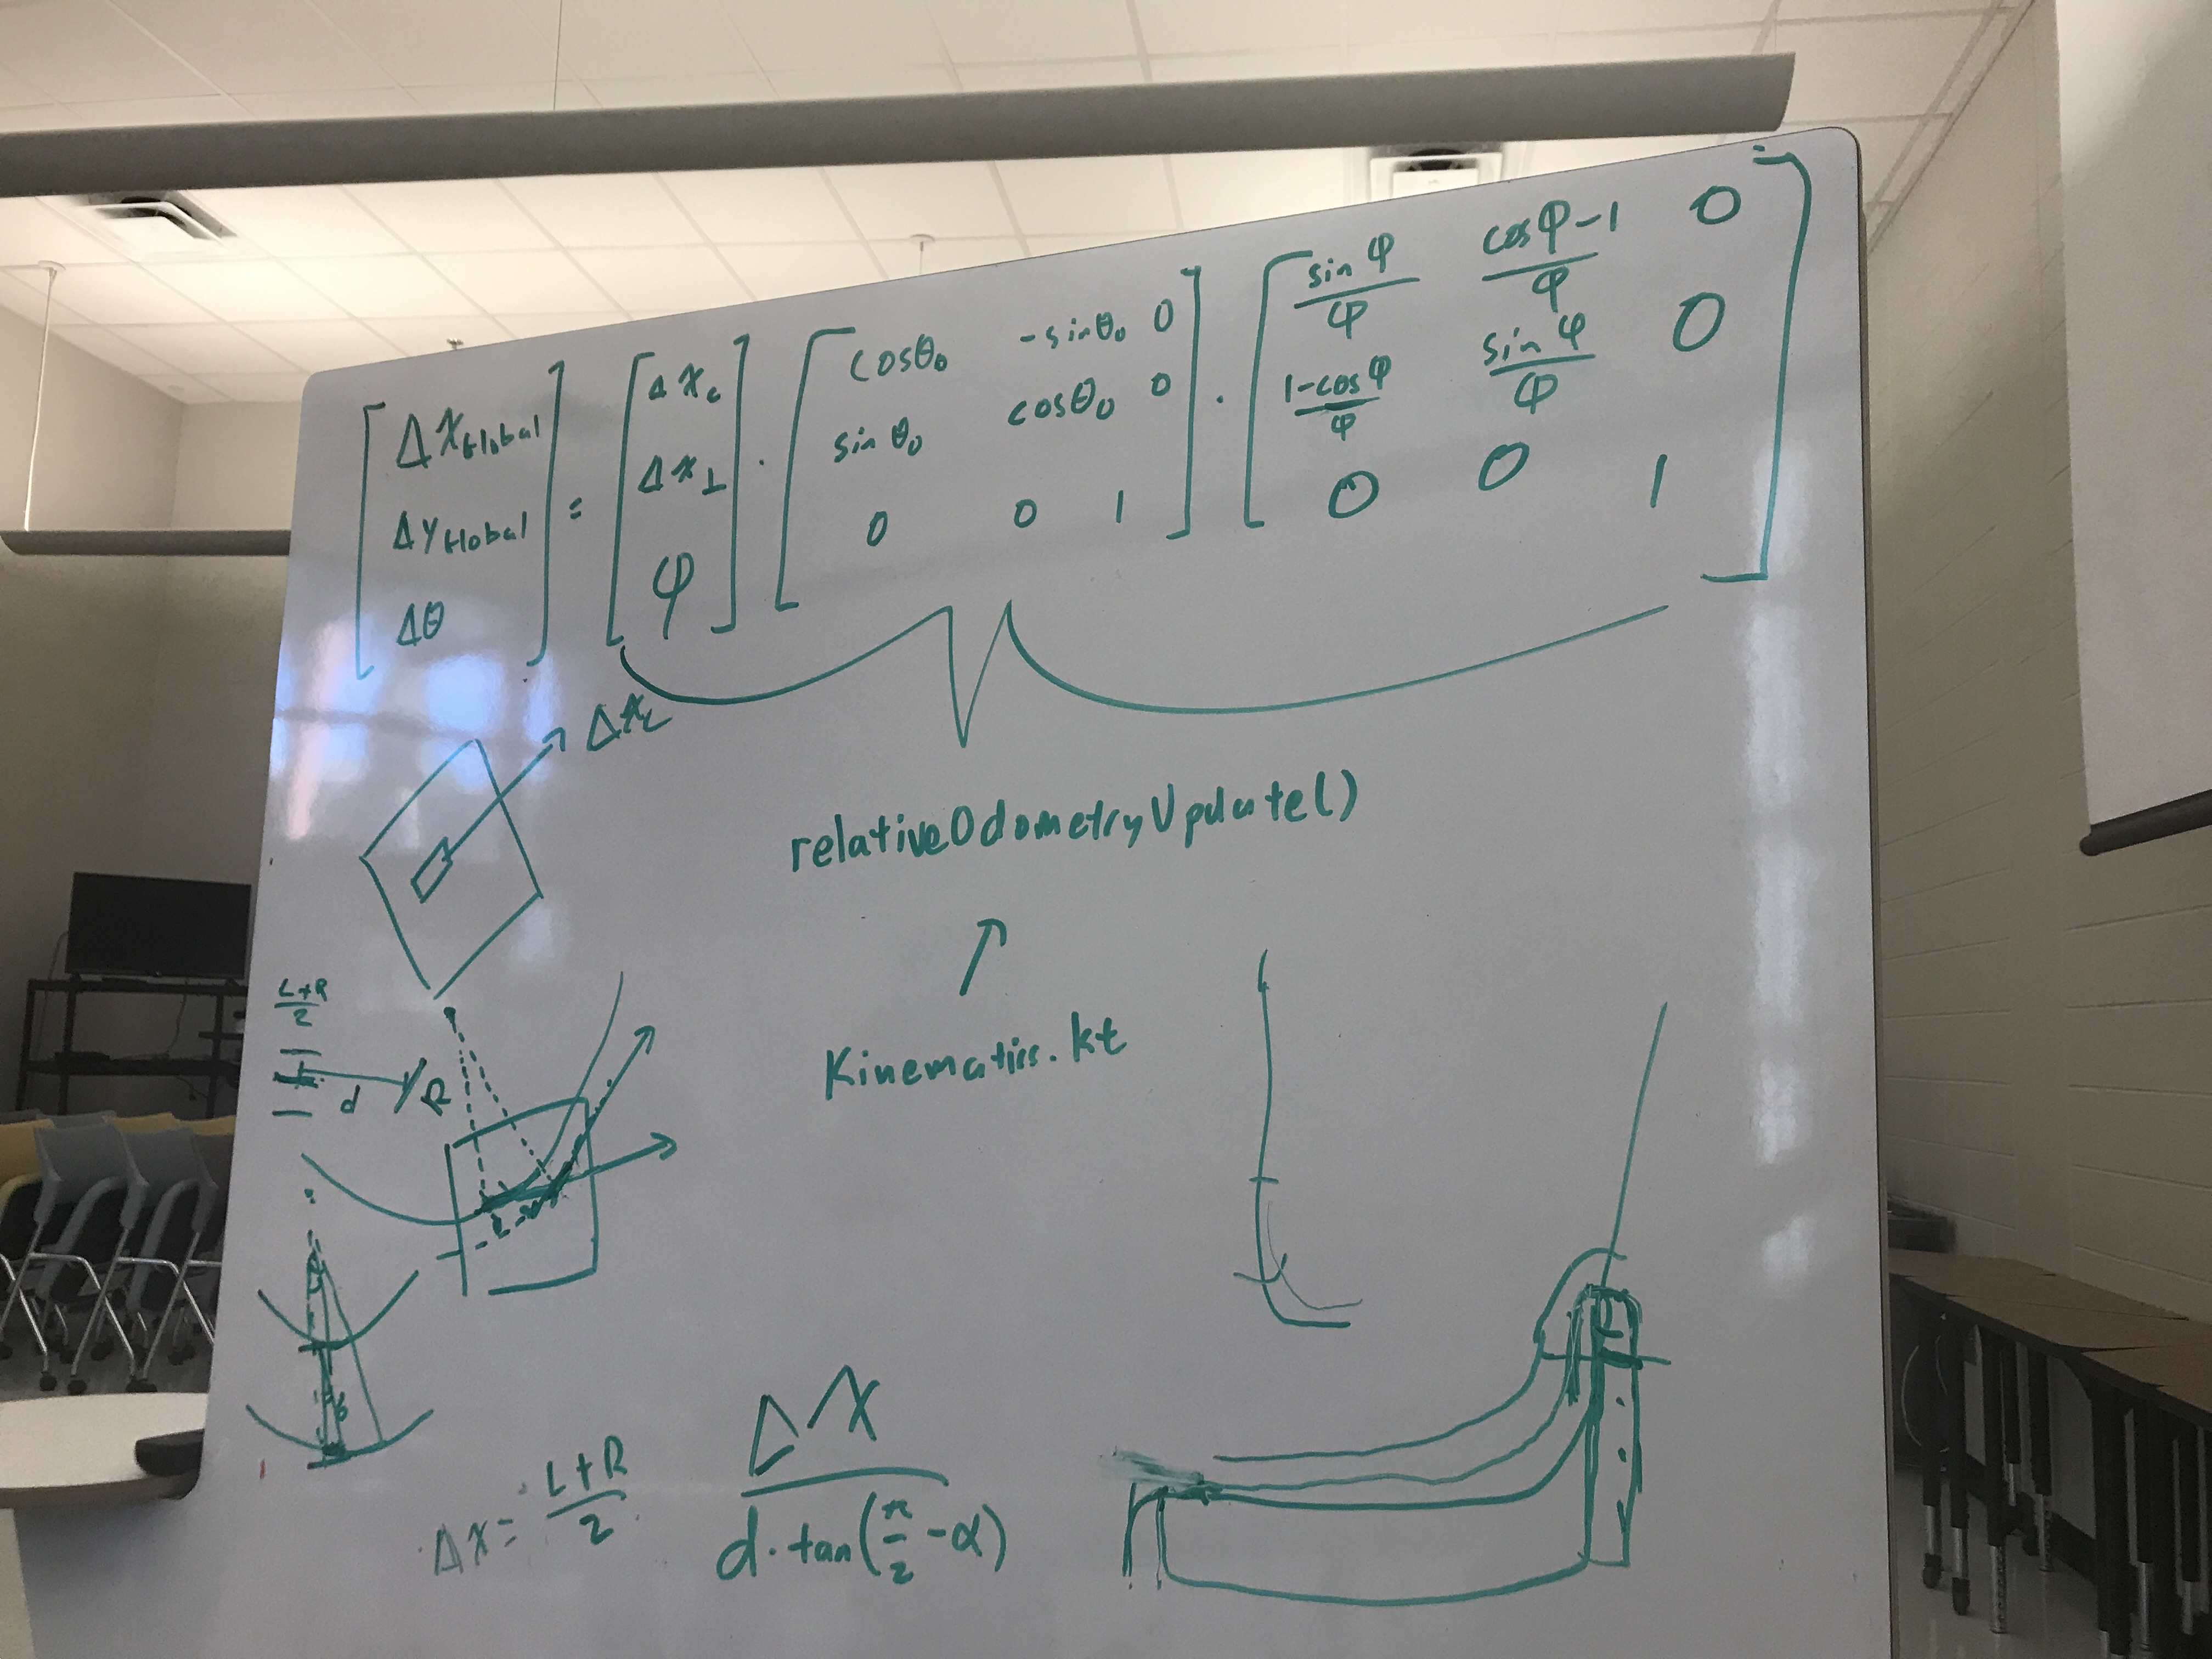
\includegraphics[width=0.95\textwidth, angle=0]{Meetings/January/01-04-22/SteeringAngletoHeadingFormula - Big Boik.JPG}
\caption{Deriving our tricycle kinematic formulas}
\label{fig:010422_1}
\end{figure}

\whatsnext{
\begin{itemize}
    \item Improve reliability of the system. 
\end{itemize} 
}

